\documentclass[a4paper,11pt,dvipdfmx]{jsarticle}
%最近はjarticleでなくjsarticleクラスを使うのが主流

%このソースファイルは以下のコマンドによりコンパイルされている
%platex -kanji=utf8 sample.tex
%dvipdfmx sample.dvi
%
%ptex2pdfコマンドを使うと，一発でplatex + pdf化を実行することもできる．
%ptex2pdf -l -ot -kanji=utf8 sample.tex

% Package Declaration
\usepackage{graphicx}

\title{ネットワーク系演習　レポートサンプル}
\author{泉 泰介(XXXXXXXXXXX)} %XXXXXXXのところには学籍番号を書くこと
\date{2018年3月28日} %ここには提出日付を書くこと

\begin{document}

\maketitle  %このコマンドでタイトルが作成される

\section{latexの基本的な取り扱い}

ここから本文を書く．表紙だけで１ページ使う必要はない．本文を書くときは
無用な改行，改段落を入れすぎないようにすること．なお，体裁や誤字，脱字，
ページ幅からのはみ出し等，内容とは直接関係ないレポートのクオリティも採点に
考慮されるので，おろそかに作成しないこと．なお，このpdfファイルのlatexによる
ソースファイルも併せてアップロードしている．ソース中にはコマンドそのほかについての
解説をコメントにて説明しているので，一読することを薦める．

\subsection{箇条書き}
箇条書きを使いたいときはitemize命令を使う

\begin{itemize}
\item 1つ目の箇条書き
\item 2つ目の箇条書き
\item 3つ目の箇条書き
\end{itemize}

箇条書きに通し番号をつけたいときはitemizeの代わりにenumerateを使う．

\subsection{ソースコードの引用}

レポートでソースコードを引用したいときは以下のようにするとよい，

\begin{quote}
\begin{verbatim}
void main(void){
    printf("Hello, World.\n");
}
\end{verbatim}
\end{quote}

\newpage

\subsection{図の貼り付け}

図の貼り付けは以下のようにすると良い．

\begin{center}
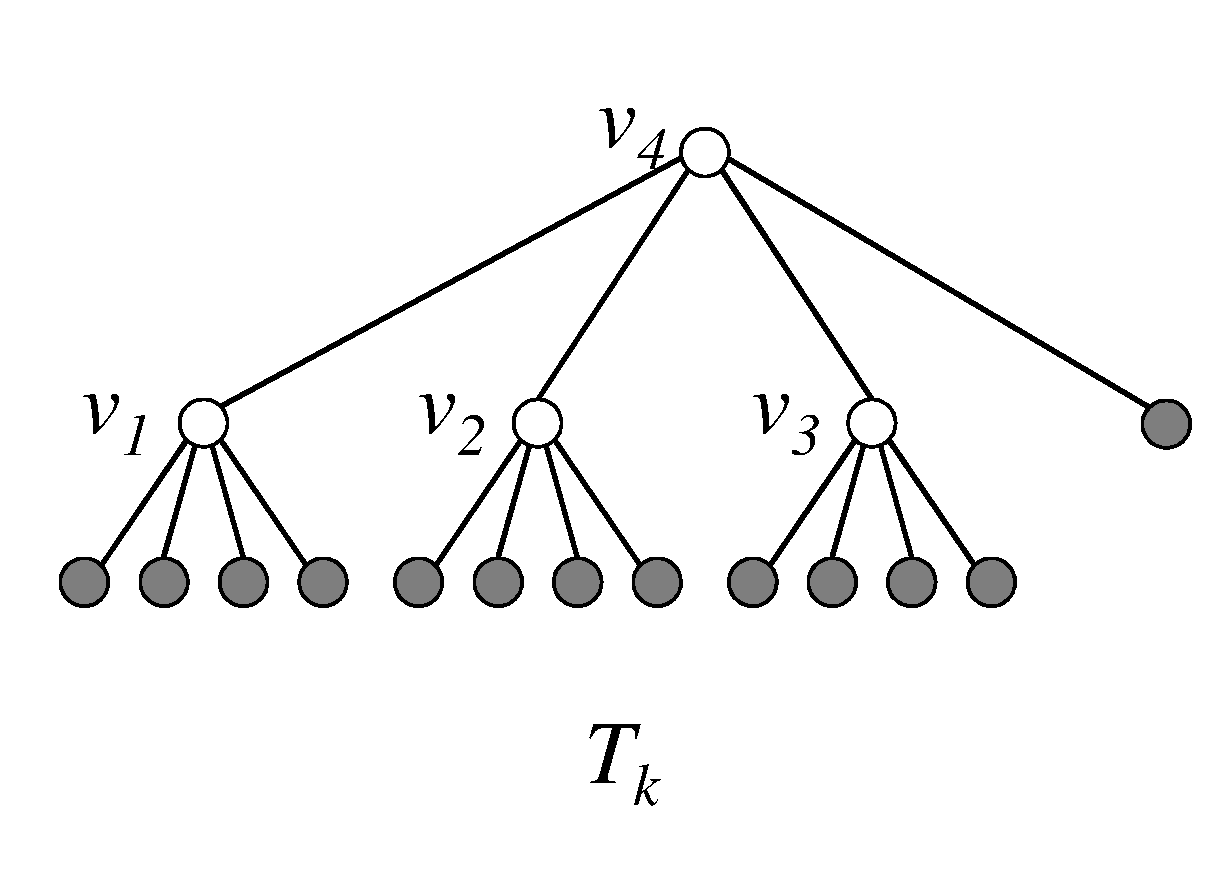
\includegraphics[keepaspectratio,width=90mm]{fig.eps}
%keepaspectratioは図の縦横比を固定する
%widthで幅の長さを指定できるので，ページから図がはみ出すときはここの
%値を調節する．その後のfig.epsは貼り付けたいファイル名を指定．
\end{center}

この例では図をeps形式に変換して貼り付けているが，最近は取り扱いのしやすさ，対応ソフトの
多さから，pdf形式での画像を張り付ける場合も多い．対象画像をpdf形式で保存した(xxx.pdfと
する)のち，
\begin{quote}
    \begin{verbatim}
%pdfcrop xxx.pdf
    \end{verbatim}
\end{quote} 
とすると，余分な余白を除外できる．

\subsection{表の作成}

表は以下のようにして作る．

\begin{center}
\begin{tabular}{|l||c|r|r|} 
%後ろの引数は各列の揃えを指定する．lが左，cが中央，rが右揃え
%揃えの指定文字の間の|は列間の罫線の有無を指定している．
%"|"だと1重，"||"だと2重罫線．何も書かなければ罫線なし．
\hline 
アルゴリズム　&  平均  & 最悪 & 最小 \\ \hline \hline 
%\hlineを置くと横罫線が引かれる  
A             &  100   &  180 & 50   \\ \hline
B             &  200   &  620 & 15   \\ \hline
C             & \multicolumn{3}{|c|}{計測不能} \\ \hline 
\end{tabular}
\end{center}

\newpage

\subsection{figure環境の利用}

図や表やソースコードにキャプションをつけてフロート表示するときは
figure環境を使う．例えば前述の図や表は以下のようになる．

\begin{figure}[!ht] 
%hはできる限り現在の位置にフロートを配置する
%tは現在の位置から近い場所のページ上部にフロートを配置する
%!は位置指定の強制力を強める(レイアウトが多少窮屈になってもできる限り指定位置に配置する)．
%!なしでうまくいかない場合，!を付ければ大体意図通りの位置に配置されることが多い．
\begin{center}
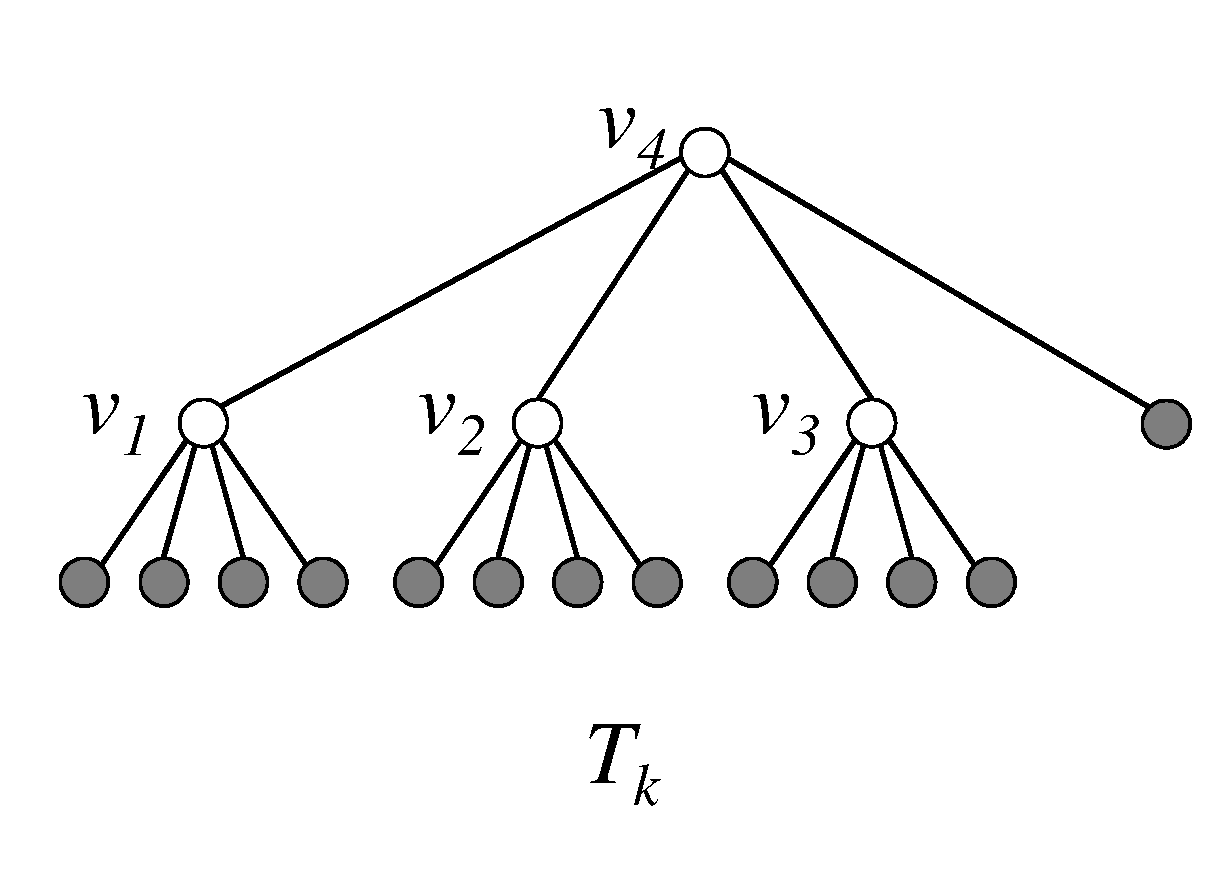
\includegraphics[keepaspectratio,width=90mm]{fig.eps}
\caption{図の例}
\label{fig:example}
\end{center}
\end{figure}


\begin{figure}[!ht]
\begin{center}
\caption{表の例}
\label{table:example}
\begin{tabular}{|l||c|r|r|} 
\hline 
アルゴリズム　&  平均  & 最悪 & 最小 \\ \hline \hline 
A             &  100   &  180 & 50   \\ \hline
B             &  200   &  620 & 15   \\ \hline
C             & \multicolumn{3}{|c|}{計測不能} \\ \hline 
\end{tabular}
\end{center}
\end{figure}

このとき，図\ref{fig:example}, 表\ref{table:example}のように
図表番号を本文で参照できる．なお，キャプションは通常，
図に対しては下側，表に対しては上側につけるのが普通である．


\subsection{横に表や図を2つ並べる}

いろいろなやり方があるが，高さ1，幅2の表の中に埋め込んでしまうという手がある(図\ref{fig:example2})．

\begin{figure}{!ht}
\begin{tabular}{cc}
\begin{minipage}{0.48\hsize}
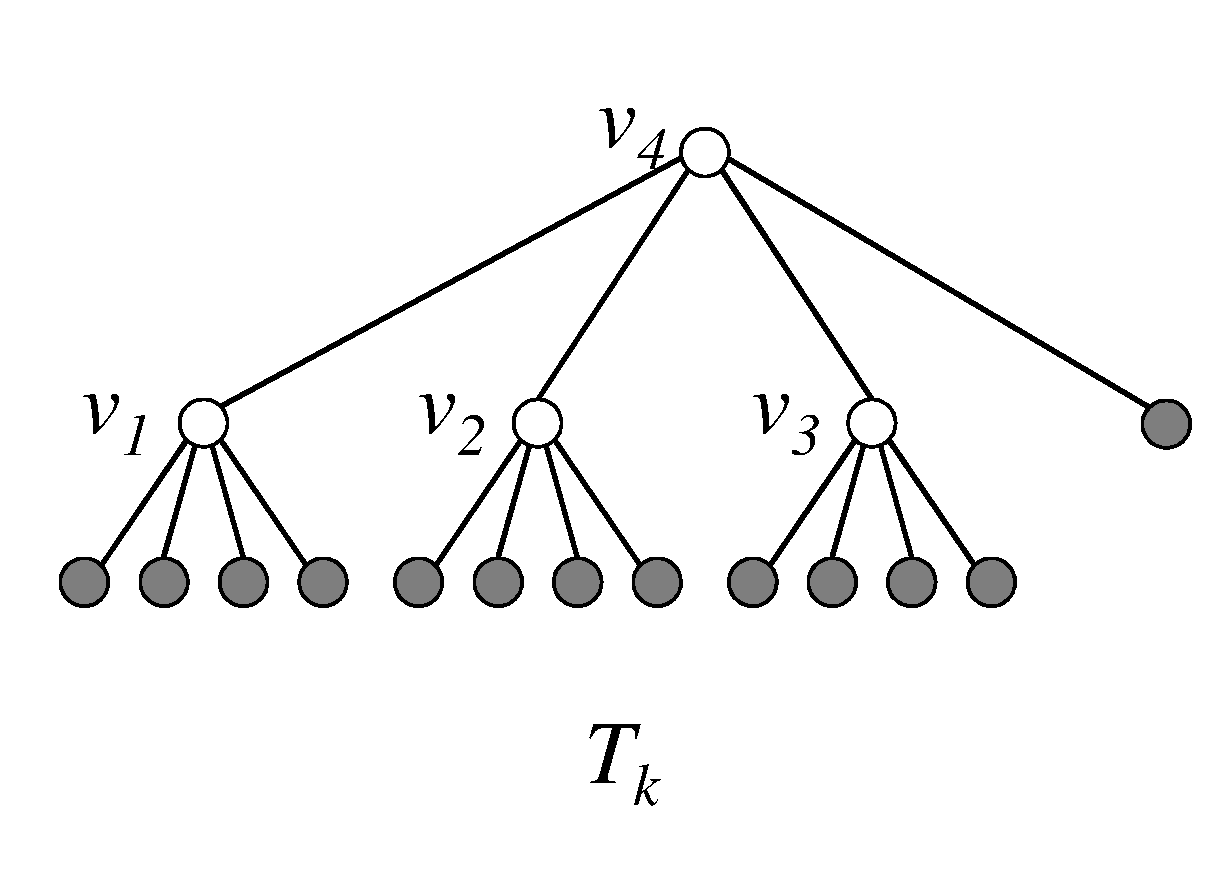
\includegraphics[keepaspectratio,width=50mm]{fig.eps} 
\end{minipage}
&
\begin{minipage}{0.48\hsize}
\begin{tabular}{|l||c|r|r|} 
\hline 
アルゴリズム　&  平均  & 最悪 & 最小 \\ \hline \hline 
A             &  100   &  180 & 50   \\ \hline
B             &  200   &  620 & 15   \\ \hline
C             & \multicolumn{3}{|c|}{計測不能} \\ \hline 
\end{tabular}
\end{minipage}
\end{tabular}
\caption{図や表を横に並べる例}
\label{fig:example2}
\end{figure}

%minipageは文章中に小さなページを入れ子で作成する命令．{0.48\hsize}は
%入れ子で作るページのサイズ指定で，元々のページ幅(=\hsize)の48%の幅の
%ページを作れ，という指定．

\section{文章作法}

レポートでは，結果だけを書くのではなく，手順，作業中に考えたこと，気をつけた
こと，その他アピールポイントなどを含めて記述すること．よく「○○を動作
させたら，正しく動作した．」とだけ書いて報告する人がいるが，課題をこなしている
以上正しく動作しているのは分かっているので，上記のような報告には意味がない．
何を伝えるべきか（何が意味のある情報なのか）ということを常に意識して作成すること．
なお，文章作法として，以下に挙げるようなレポートは禁止である．
\begin{description}
\item[本文がなく，ほとんど箇条書きのみで報告する]
レポートに限らず，「文書としてまとめる」ということは，
基本的には平文で記述するということである．箇条書きは
書くのが楽なので，ついつい多用しがちであるが，本当に箇条書きで
書く必要がある内容なのかどうか，考えて使うこと．箇条書きで
書くと便利な内容の代表例は(1)列挙(複数の並立するものを述べる)，
(2)手続き(順番が意味を持つないような直列の内容)であるが，
逆に言うと，それ以外では利用する必要性はあまりない．
\item[改行，章節の区切りをやたらと多用する]
ほとんど一文おきに改行する人がいるが，日本語，英語問わず，
改行(改段落)は「(ある程度まとまった単位での)意味の区切り」を示す
ためのものである．意味もなく改行しないこと．
また，意味をふまえて改行を入れた上で，それでも各段落が細かく
なってしまう場合は，文章のまとまりを少し細かく区切り過ぎている
可能性が高い．接続詞を入れたり，文章を書き換えて改行前後の話の
つながりを分かりやすくするなどして，文章がもう少し大きくまとまる
ようにすること．また，改行，改段落と同じ効果を意図して，章番号，
節番号でやたらと細かく内容を区切る人がいるが，これもやり過ぎは
かえって読みにくいので，本当にその区切りが必要か再考すること．
たとえば，本文が一，二文しかないような節は，必要のない可能性が高い．
\item[考察と感想を混同する] レポートである以上課題を行う上で
考えたことは記載する必要があるが「大変だった」「楽しかった」などの
個人的な気持ちについての感想を考察の一部として記載してはいけない．
基本的には報告書に感想を書く必要はないが，書きたい場合は，
たとえばレポートの最後に別途記載する等，報告部分と明に切り離して
書くこと．
\item[余計なことをたくさん書く] たとえば，演習の手引きに既に書いている
内容の一部をまるまるコピーしてレポートに書く人がいるが，無駄である．
ページ数を増やすために行っているのかも知れないが，ページ数は評価と
無関係なので，無理に余計なことを書いて水増しする必要はない．
報告内容を``過不足なく簡潔に書く''ことが良いレポートの条件であると
心得ること．ただし，レポート自体はあくまで(演習手引き書なしで)レポート
単体で読める必要があるので，「演習手引きに書いてあるので省略」して
いいわけではない．重要なことは「手引き書の内容を書くな」ということ
ではなく「手引き書の内容を（必要もないのに）丸写しするな」ということ
である．自身の報告に必要であれば，適宜内容を引いてくること．
\item[過度な修辞] 報告書は小説や随筆ではないので，名文を書く必要はない
．流麗だが誤解を招く文章より，多少ぎこちなくとも，意味の通った，
あいまいさのない文章であるほうが良い．
\end{description}

\end{document}
